\chapter{Part III: The Art of Listening}

This chapter follows the movement of a dialogue between J. Krishnamurti and Dr. Alan W. Anderson on seeing, listening, learning, attention, and freedom. Its exactness is not algebraic in the usual sense, but the structure is rigorous. Krishnamurti asks us to distinguish direct perception from perception mediated by memory, image, belief, reward, and time. We will keep the spoken order of the inquiry and use a few compact schemas only as aids for seeing the movement more clearly.

\section{The Question of Seeing}

Anderson opens by recalling where the previous conversation had ended: beauty had led them to the question of seeing and to the transformation of human beings, a transformation not dependent on knowledge or time. Krishnamurti immediately widens the question. What is seeing? What is listening? What is learning? These are not separate topics placed side by side. They will turn out to be interrelated movements.

The first question is whether we actually see. We may suppose that seeing is obvious: the eye is open, the object is present, and perception occurs. Krishnamurti interrupts that assumption. What we call seeing may be seeing through a screen: prejudice, idiosyncrasy, experience, wishes, pleasures, fears, and the images we hold about the thing and about ourselves.

Let \(M\) denote the perceiving mind, \(O\) the object perceived, and \(S_1,\ldots,S_n\) the screens through which the mind looks. The following is not source notation; it is a compact reconstruction of the spoken distinction:
\begin{equation}
M \xrightarrow{\;S_1,S_2,\ldots,S_n\;} O .
\end{equation}
The point is not that perception is a mechanical pipeline. The point is that the thing may never be met directly. The mind may be meeting its own memories, its botanical knowledge, its belief, its fear, or its image of the thing.

\begin{definition}
A \emph{screen} is any image, conclusion, belief, memory, prejudice, fear, pleasure, or accumulated experience that stands between the mind and what is being perceived.
\end{definition}

This gives the first pressure of the chapter: seeing may not take place at all. What we call seeing may be recognition, naming, comparison, expectation, or the operation of the past.

\begin{figure}
\centering
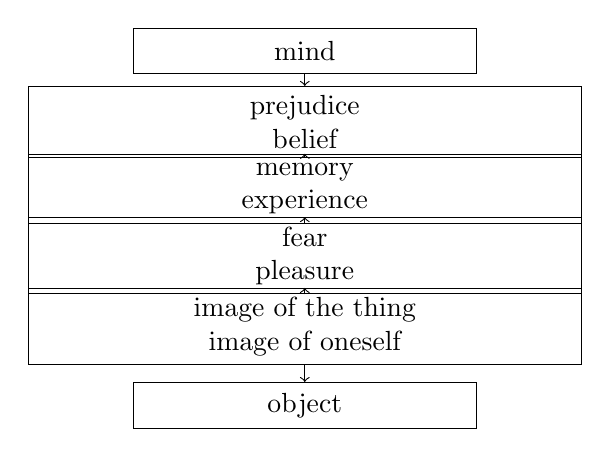
\begin{tikzpicture}
\node[draw, align=center, text width=0.34\linewidth, minimum height=0.58cm] (mind) at (0,4.15) {mind};
\node[draw, align=center, text width=0.56\linewidth, minimum height=0.58cm] (s1) at (0,3.25) {prejudice\\belief};
\node[draw, align=center, text width=0.56\linewidth, minimum height=0.58cm] (s2) at (0,2.4) {memory\\experience};
\node[draw, align=center, text width=0.56\linewidth, minimum height=0.58cm] (s3) at (0,1.55) {fear\\pleasure};
\node[draw, align=center, text width=0.56\linewidth, minimum height=0.68cm] (s4) at (0,0.65) {image of the thing\\image of oneself};
\node[draw, align=center, text width=0.34\linewidth, minimum height=0.58cm] (object) at (0,-0.35) {object};
\draw[->] (mind) -- (s1);
\draw[->] (s1) -- (s2);
\draw[->] (s2) -- (s3);
\draw[->] (s3) -- (s4);
\draw[->] (s4) -- (object);
\end{tikzpicture}
\caption{A transcript-based reconstruction of the ``screen after screen'' movement in perception.}
\end{figure}

The question then becomes sharper: can the mind look without those screens? Not as a method, not as practice, but simply as a fact to be investigated. Can there be looking without image, conclusion, belief, memory, prejudice, and fear?

\section{Seeing and Action}

The inquiry does not remain with perception as a private state. Once seeing is raised, action appears. Krishnamurti says that when there is a seeing of the thing, there is no question of postponement, succession, or interval. We can record the structural claim as
\begin{equation}
\hbox{direct seeing}
\Rightarrow
\hbox{action without interval}.
\end{equation}
This is not a behavioral formula. It preserves the distinction the dialogue is making: direct seeing is not followed by a separate operation in which an idea is selected, carried forward, and implemented.

The contrast is action based on a belief, conclusion, idea, or formula:
\begin{equation}
\hbox{belief/conclusion/idea}
\Rightarrow
\hbox{time-binding action}
\Rightarrow
\hbox{conflict and sorrow}.
\end{equation}
``Time-binding'' here means bound to interval: postponement, succession, regret, and consequence. The action begins from a formula; the formula belongs to knowledge; knowledge belongs to the past. The past then acts under the name of present action.

\subsection{Question \& Answer}

\paragraph{Question.}
If action is not based on an idea, how does action occur?

\paragraph{Answer.}
The lecture's answer is that action is not separate from seeing. If the danger, falseness, or fact is seen directly, action is already in that seeing. The interval appears only when seeing is replaced by belief, conclusion, or formula. Anderson later gives the concise phrase: the action and the seeing are one act.

A useful reconstruction is
\begin{align}
\hbox{direct seeing} &\Rightarrow \hbox{no interval},\\
\hbox{idea-based action} &\Rightarrow \hbox{interval and conflict}.
\end{align}
The distinction is local and precise. Krishnamurti is not saying that practical knowledge has no place. He is saying that when psychological action is based on an idea, it carries division and time into the action itself.

\section{Listening Without Interference}

From seeing, the dialogue turns to hearing. The same structure returns in the field of relationship. Do we ever hear another person directly, or do we hear through the image built about that person? We may hear a wife, husband, friend, or stranger through irritation, annoyance, domination, conclusion, and remembered injury. The voice is present, but the mind listens through its own accumulated relationship.

Anderson recalls a remark from an earlier conversation: hearing is doing nothing to stop or interfere with seeing. That remark is important because it reverses the ordinary idea of hearing. We usually treat hearing as effort: lean forward, concentrate, obey the command to ``hear me out.'' Krishnamurti is pointing in the opposite direction. Listening is not produced by strain. It appears when interference is absent.

Let \(L\) stand for the act of listening and \(I\) for interference: translation, interpretation, conclusion, comparison, agreement, disagreement, like and dislike. The reconstructed bookkeeping relation is
\begin{equation}
L_{\rm direct}=L-I .
\end{equation}
This is not a measured equation. It is a reminder that in this dialogue listening is clarified by subtraction. We do not add intensity in order to listen; we see the movements that prevent listening.

The next question is the pivotal one: what happens when a statement is actually heard?

\section{The Abstraction Loop}

Krishnamurti chooses a concrete statement from the prior inquiry: beauty cannot be understood apart from suffering and passion. The ordinary mind hears such a statement and almost immediately turns it into an idea. It hears words, draws a conclusion, forms a verbal abstraction, and then asks how to carry that idea out. At that moment the statement has become a problem.

We can write the ordinary movement as an update sequence:
\begin{equation}
\hbox{statement heard}
\to
\hbox{words}
\to
\hbox{conclusion}
\to
\hbox{idea}
\to
\hbox{problem of carrying it out}.
\end{equation}
This is the chapter's cleanest local mechanism. The mind has not stayed with the statement. It has converted the statement into its own abstraction. Once different minds carry different abstractions, conflict follows naturally.

\begin{proposition}
When a statement is converted into an idea, the mind no longer listens to the statement directly; it deals with the abstraction it has made from the statement.
\end{proposition}

\begin{proof}
The spoken sequence supplies the steps. First, the statement is heard as words. Second, the mind draws a conclusion. Third, the conclusion becomes an idea. Fourth, the mind asks how that idea is to be carried out. The practical problem therefore belongs to the abstraction, not to direct listening. Thus the mind has shifted from listening to the statement to managing its own construction.
\end{proof}

\subsection{Question \& Answer}

\paragraph{Question.}
What happens when a statement is heard without abstraction?

\paragraph{Answer.}
The answer is not that the mind reaches a more refined conclusion. It does not compare, agree, disagree, translate, or form an idea. It listens completely. In that complete listening there is attention, and in attention the truth or falseness of the statement is seen in the statement itself.

The contrast is:
\begin{align}
\hbox{ordinary hearing}
&:\quad
\hbox{statement}\to\hbox{idea}\to\hbox{problem},\\
\hbox{complete listening}
&:\quad
\hbox{statement}\to\hbox{attention}.
\end{align}
This is why the lecture's rhythm must be preserved. Krishnamurti does not begin with attention as an ideal. Attention is discovered by watching what the mind does to a statement.

\section{Attention Without Reward}

Attention is now the center of the inquiry. Krishnamurti says that attention means no border. The moment there is a frontier, the mind begins to fight, agree, disagree, compare, and form concepts. We may record the border condition as
\begin{equation}
\hbox{frontier in attention}
\Rightarrow
\hbox{concept, comparison, resistance}.
\end{equation}
The absence of frontier is not vagueness. It is the condition in which the mind is not divided from what is being heard.

Anderson then offers a lived example from the filmed conversations themselves. He has had to attend to the conversation while the practical machinery of production continues. Yet when the conversation is deeply engaged, the mechanism is carried on more efficiently, not less. Krishnamurti takes the example into a more general exposure: the mind lives in the marketplace. It asks for exchange. I give this; you give that. I practice; I receive a result. Even religion can become commerce.

That is why the question ``How shall I maintain attention?'' is already suspect. It asks for a method that will secure a return:
\begin{equation}
\hbox{practice attention}
\to
\hbox{obtain reward}.
\end{equation}
But Krishnamurti says attention is not a result. It has no cause in the reward-seeking sense. What has a cause has an effect, and the effect becomes a further cause. That is a circle, while attention does not belong to that circle.

\begin{figure}
\centering
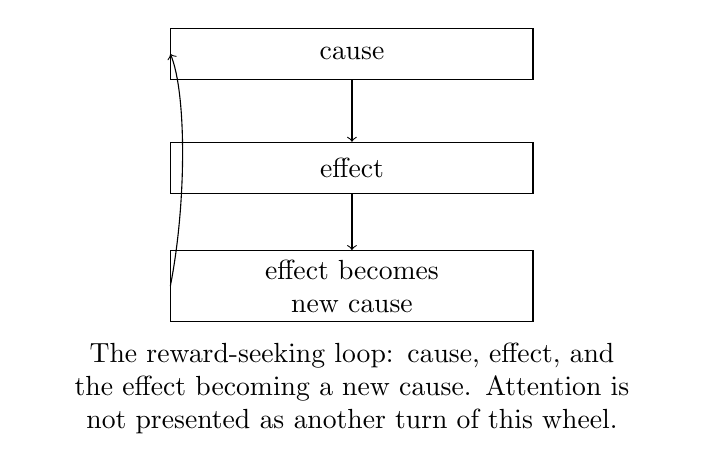
\begin{tikzpicture}
\node[draw, align=center, text width=0.36\linewidth, minimum height=0.65cm] (cause) at (0,2.8) {cause};
\node[draw, align=center, text width=0.36\linewidth, minimum height=0.65cm] (effect) at (0,1.35) {effect};
\node[draw, align=center, text width=0.36\linewidth, minimum height=0.75cm] (newcause) at (0,-0.15) {effect becomes\\new cause};
\draw[->] (cause) -- (effect);
\draw[->] (effect) -- (newcause);
\draw[->] (newcause.west) .. controls (-2.1,0.9) and (-2.1,2.3) .. (cause.west);
\node[align=center, text width=0.66\linewidth] at (0,-1.45) {The reward-seeking loop: cause, effect, and the effect becoming a new cause. Attention is not presented as another turn of this wheel.};
\end{tikzpicture}
\caption{A narrow reconstruction of the cause-effect circle discussed in relation to reward and attention.}
\end{figure}

The lecture is careful here. It does not give a method for attention. It shows why the search for a method may already be the movement of reward.

\section{Learning and the Mechanical Mind}

The inquiry now pivots from seeing and hearing to learning. Krishnamurti explicitly says that seeing, hearing, learning, and action are interrelated. They are not separate chapters; they are one movement. So the question becomes: what is learning?

The first answer is ordinary and necessary. We learn a language. We learn to ride a bicycle, drive a car, put together a machine, practice a craft, and earn a livelihood. This is learning as accumulation, and it has its proper field. Let \(K_{\rm mech}\) denote this practical field of mechanical knowledge:
\begin{equation}
\hbox{experience}+\hbox{knowledge}
\to
\hbox{memory}
\to
K_{\rm mech}
\to
\hbox{routine action}.
\end{equation}
This is not dismissed. It is indispensable. The question is whether psychological or inward learning is of the same kind.

\begin{definition}
\emph{Mechanical learning} is learning as accumulation: experience stored as memory and used as skill, routine, profession, or practical function.
\end{definition}

The inquiry becomes severe when Krishnamurti asks whether we learn from experience. If human beings had learned in the deeper sense, repeated sorrow and repeated war would have ended. Yet the repetition continues. The transcript's test can be written:
\begin{align}
\hbox{repeated sorrow}
&\not\Rightarrow
\hbox{freedom from sorrow},\\
\hbox{repeated war}
&\not\Rightarrow
\hbox{freedom from war}.
\end{align}
So the claim is not that experience has no technical value. It is that experience, stored as memory, has not transformed the movement of the mind. It has produced repetition, security, and routine. Education, culture, and civilization have trained the brain to function mechanically.

The phrase ``known to known'' summarizes this movement:
\begin{equation}
\hbox{known}\to\hbox{known}
\Rightarrow
\hbox{movement in time}
\Rightarrow
\hbox{not freedom}.
\end{equation}
Thought is always old in this sense. It may rearrange, add, subtract, and recombine, but it is still moving within the known.

\subsection{Question \& Answer}

\paragraph{Question.}
Is there any non-mechanical learning?

\paragraph{Answer.}
Krishnamurti does not answer by adding a higher spiritual curriculum to the ordinary one. That would still be accumulation. One can learn a language, a craft, or a technical skill. One can also learn about oneself as the known, because the self is the accumulated past: fear, envy, success, regret, belief, invented soul, invented image of God. But to learn about God, freedom, or the inward as though these were objects added to knowledge is still mechanical.

So the question turns back on itself. If there is no other learning in the accumulative sense, what takes place? The answer begins with understanding the movement of knowledge itself. Where knowledge ends, or where the mind sees the limit of knowledge, the question of freedom can begin.

\section{Knowledge, Silence, and Meditation Deferred}

The later part of the dialogue asks what happens when the mind understands the whole field of knowledge. Anderson brings in Vedanta as the end or consummation of knowledge, but Krishnamurti keeps the emphasis practical: the mind knows the activity of the known. The question is the state of a mind that is free from that activity and yet functions in knowledge.

This is the deepest apparent contradiction in the lecture:
\begin{equation}
\hbox{functioning in knowledge}
\neq
\hbox{bondage to knowledge}.
\end{equation}
We need knowledge to speak, drive, build, teach, and carry out ordinary tasks. The problem is not practical functioning. The problem is the mind's psychological bondage to the known, where even seeing and listening become mechanical.

Krishnamurti then asks whether there is listening out of silence. In that silence there is no wanting, no reward, no punishment, no project of self-improvement. He identifies that listening with attention:
\begin{equation}
\hbox{silence}+\hbox{listening}
\Rightarrow
\hbox{attention not bound to time}.
\end{equation}
Anderson notices that meditation, in this sense, is not something done in succession. Krishnamurti does not expand the subject here. He says meditation must be gone into deeply another time, partly because the word has been damaged by technique, schedule, payment, and the idea that meditation is something one learns as another acquisition.

Then comes an important recap. They began with beauty, then passion, suffering, action, seeing, and hearing. Action based on idea is inaction. Seeing and listening have become mechanical when they move only from the known to the known. Freedom, if reduced to an idea, remains within knowledge. But when the movement of knowledge is understood, another question becomes possible: can one observe out of silence and act in the field of knowledge, both together in harmony?

\section{Words and the Thing}

Before the close, Anderson describes a teaching situation in which students could think about a doctrine but hesitated when asked to look directly. Krishnamurti draws the lesson back to words. We are caught in words; the word is not the thing. The description is not the described. Yet the description often becomes all that matters.

This belongs to the same architecture as the screens. The word can become a screen:
\begin{equation}
\hbox{word} \neq \hbox{thing}.
\end{equation}
When the word becomes dominant, the door named by the word disappears behind the name. Education and philosophy can strengthen this abstraction: theorizing endlessly about how one should live while not living it.

The movement can be written:
\begin{align}
\hbox{thing}
&\to
\hbox{word}
\to
\hbox{abstraction}
\to
\hbox{theory},\\
\hbox{direct seeing}
&\to
\hbox{appropriate action}.
\end{align}
This final contrast returns us to the beginning. The problem is not language as a practical tool. The problem is the mind's enslavement to the word, the image, the concept, and the abstraction, so that the thing itself is never met.

\section{Summary}

The art of listening, in this dialogue, is not a technique for becoming a better listener. It is part of a single inquiry into seeing, hearing, learning, action, knowledge, and freedom. Seeing through screens is not seeing. Hearing through image and conclusion is not listening. Action based on idea is time-binding. Attention is not produced by cause, reward, or practice. Mechanical learning is necessary in its field, but it does not answer the deeper question of freedom.

The chapter's negative map is:
\begin{equation}
\hbox{screens}
\to
\hbox{abstraction}
\to
\hbox{time-binding action}
\to
\hbox{conflict}.
\end{equation}
Its counter-movement is:
\begin{equation}
\hbox{silence}
\to
\hbox{attention}
\to
\hbox{direct seeing/listening}
\to
\hbox{action without interval}.
\end{equation}
These are not formal psychological equations. They are compact reminders of the lecture's order. Krishnamurti begins with perception and ends at the edge of meditation, but he does not let meditation become method. The final question is exacting: can the mind understand the movement of knowledge, observe out of silence, and act in the field of knowledge without being bound by it?